\documentclass[uplatex]{jsarticle}
\usepackage[dvipdfmx]{graphicx}
\usepackage{ascmac}
\usepackage{listings}
\usepackage{amsmath}
\usepackage{bm}
\usepackage{cases}

\DeclareMathOperator*{\minimize}{minimize}


\title{人工知能 課題番号1「人工知能の実現可能性について考察せよ」}
\author{工学部電子情報工学科 03-175001 浅井明里}

\makeatletter
\def\maketitle{%
  \null
  \thispagestyle{empty}%
  \vfill
  \begin{center}\leavevmode
    \normalfont
    {\LARGE \@title\par}%
    \vskip 1cm
    {\Large \@author\par}%
    \vskip 1cm
    {\Large \@date\par}%
  \end{center}%
  \vfill
  \null
  \@thanks%\vfil\null
  \cleardoublepage
  }
\makeatother


\title{人工知能 課題番号23「ニューラルネットの応用例」}
\author{工学部電子情報工学科 03-175001 浅井明里}
\date{\today}

\begin{document}
\maketitle

% \section{モンテカルロ探索法とは}
% \subsection{モンテカルロ探索法と従来の手法との相違点}

\section{ニューラルネットを用いてSpeed Dating問題を解く}
本課題では、Pythonの標準ライブラリ及びNumpyを用いて二層のニューラルネットワークモデルを実装し、
このモデルを用いてSpeed Dating問題を解いた。データセットについては講義サイトで公開されている前処理済みの
full\_matching.csvを用い、この70\%を学習データセットとして学習し、残りのテストデータセットでマッチングが成立するかどうかを二値分類して
予測した。実装したニューラルネットを用いた予測の正答率は83\%程度であり、また特徴選択を行ない、正解ラベルと
相関の大きい上位20項目のみを用いた場合の予測正答率は85\%程度を達成した。

\section{ニューラルネットワークの実装}
\subsection{実装したモデル}
今回は元々のSpeed Datingデータセットの数及び入力の次元がそこまで多くないため、二層のシンプルなニューラルネットワークを実装した。
ネットワークは以下の図1のような構造となっている。
\begin{figure}
  \begin{center}
    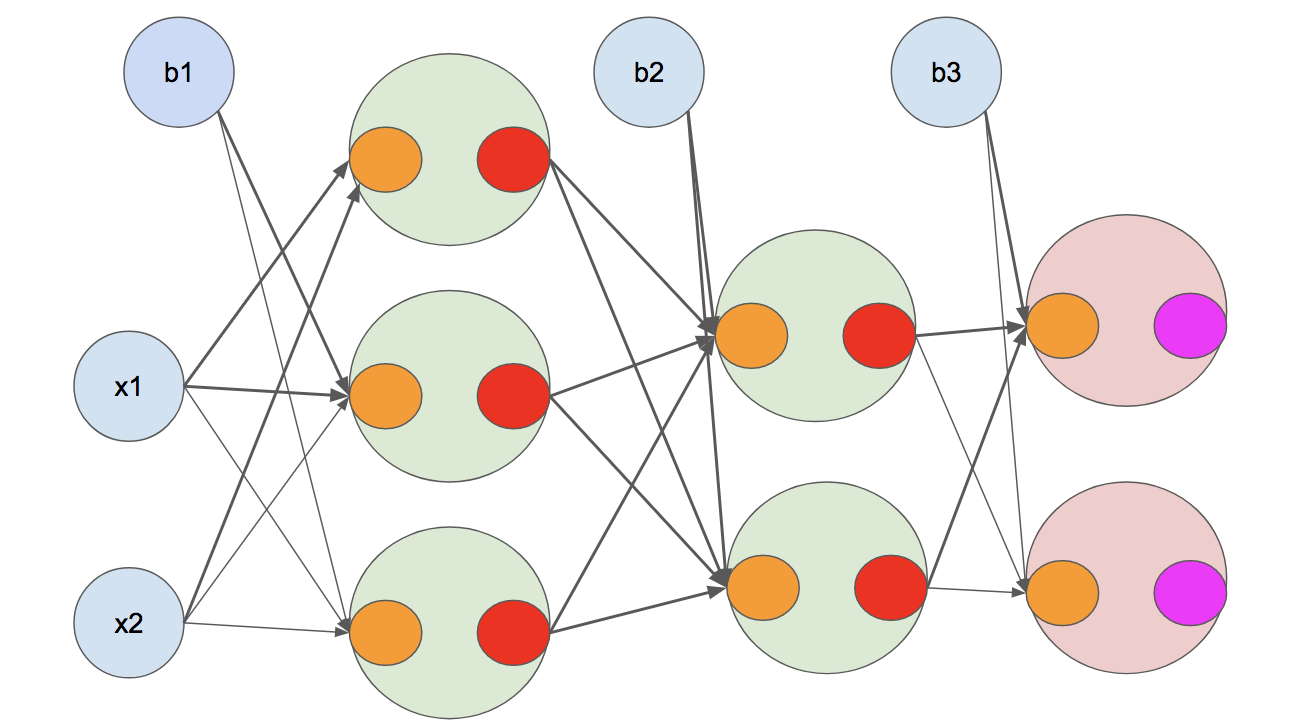
\includegraphics[width=13cm]{img/model.png}
    \caption{二層ニューラルネットワークの構造}
  \end{center}
\end{figure}
まず一層目では、それぞれのニューロンに対して、重み付き和を計算する(図の1段目の緑色のニューロンの中の橙色の部分)。
$$A ^ {(1)} = XW^{(1)} + B^{(1)}$$
次に、活性化関数にこの重み付き和を入力し、出力を次の層へ渡す(図の赤色の部分)。実験ではこの活性化関数について、
Sigmoid及びReLUで検証を行なった。
$$Z ^ {(1)} = Activation(A ^ {(1)})$$
同様のことをもう一層繰り返す。
3段目の桃色のニューロンは出力層となっており、まず一つ前の層の出力を入力として重み付き和を計算する。
$$A ^ {(3)} = Z^{(2)}W^{(2)} + B^{(2)}$$
次にこの$A ^ {(3)}$についてソフトマックス関数を適用する。
$k$番目の出力$y_k$は以下の式で求めることができる。
$$y_k = \frac{\exp{(a_k)}}{\sum_{i=1}^n\exp{(a_i)}}$$
ソフトマックス関数は0から1.0の実数になり、また出力の総和は1になる。つまりこの出力はそれぞれの出力ラベルが
どこまで確からしいかという確率として解釈できる。
このソフトマックス関数の損失関数として交差エントロピー誤差を用い、この損失関数の勾配を求め、
パラメータを勾配方向に微笑寮だけ更新することを繰り返して学習を行なった。
また勾配計算に当たって数値微分ではなく誤差逆伝播法(Back Propagation)を用いた。

\subsection{実装の詳細}
図2はディレクトリ構成を示している。
\begin{figure}
  \begin{center}
    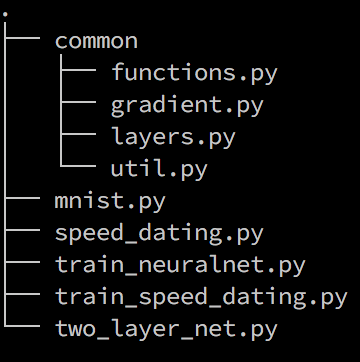
\includegraphics[width=8cm]{img/directory.png}
    \caption{ディレクトリ構成}
  \end{center}
\end{figure}
speed\_dating.pyにおいてデータの読み込みや正解ラベルのワンホットベクトル化などの処理を行いデータセットを作成し、
train\_speed\_dating.pyでtwo\_neural\_net.pyで定義された二層ニューラルネットワーククラスのインスタンスを生成し、任意のエポック数だけ学習を行う。\\
common以下の各ファイルでは誤差伝搬法で用いるレイヤクラスの定義、勾配計算及や活性化関数の定義などを行なっている。
なお、多層ニューラルネットワークの実装、誤差伝播法の実装についてはStanford大学の「CS231n: Convolutional Neural Networks for Visual Recognition
Spring 2017」講義資料等を参考にした。

実装に誤りがないか確認するため、一般に多層ニューラルネットモデルであれば95\%以上の精度を出すことができると
されているmnistデータセットに対する実験を行なった結果、最終的に97\%を超えるtest sccuracyを達成した。
図3はmnistデータセットを用いた学習でlossがエポック数に応じてどう変化したかを可視化したグラフであり、
学習が進むにつれて損失が小さくなっていることが確認できる。
\begin{figure}
  \begin{center}
    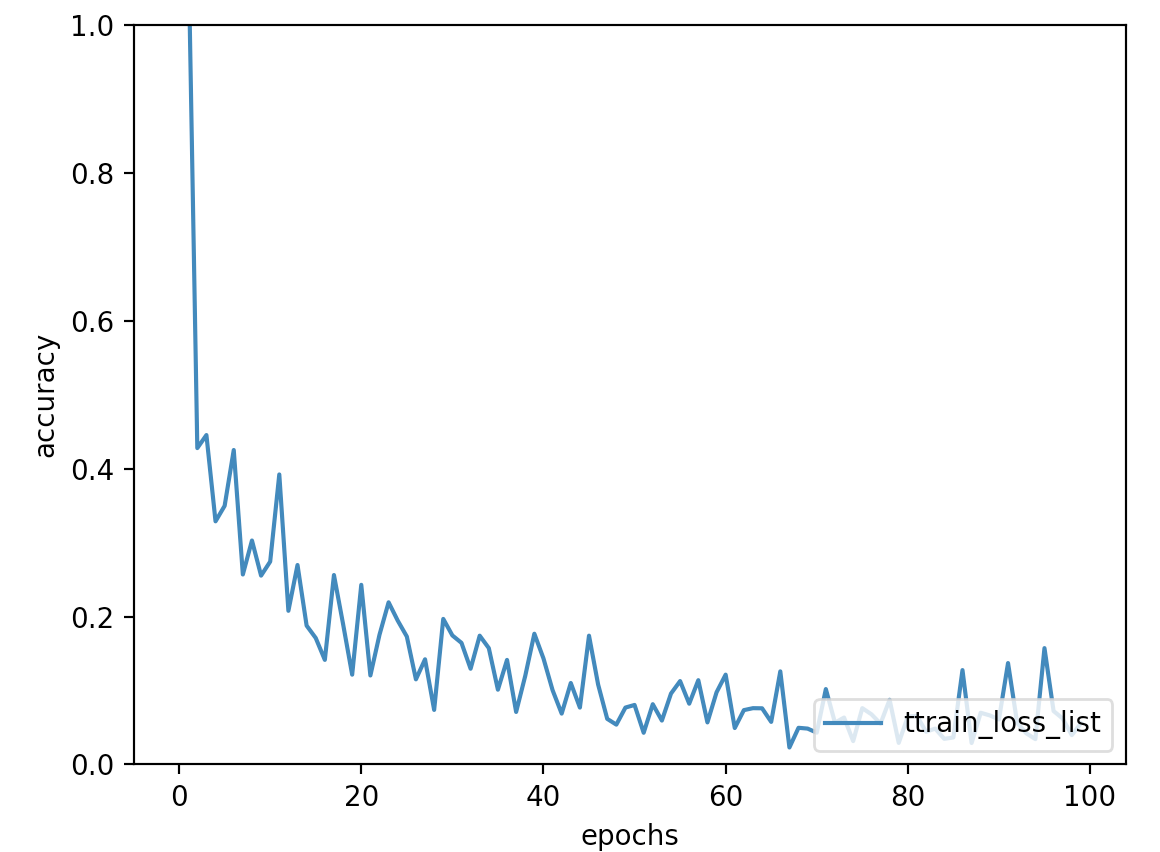
\includegraphics[width=8cm]{img/mnist.png}
    \caption{mnistデータセット学習時の損失の推移}
  \end{center}
\end{figure}

\subsection{プログラムの実行}
プログラムを実行する際にはspeed\_datingディレクトリ以下で以下のコマンドを入力すれば実行できる。
学習中はtrain及びtest accuracy, lossがepoch数の経過とともに
表示され、また学習終了時にlossの推移の様子などを可視化したグラフが表示される。
またspeed\_datingについてはspeed\_dating.pyのデータへのパスが私のマシンでの
絶対パスとなっているため、相対パスなどへの変更が必要である。
\begin{lstlisting}[basicstyle=\ttfamily\footnotesize, frame=single]
  $ python3 train_speed_dating.py
  $ python3 train_mnist.py 
\end{lstlisting}

\section{full\_matching\_dataにおける特徴選択}
full\_matching\_dataはそれぞれの男女ペアについて、マッチしたかどうかを表すmatchを除くと174項目の情報が与えられている。
ニューラルネットワークモデルを用いて予測を行うのにあたってこれらの入力を全て使うのではなく、実際にラベルとなんらかの相関のある
項目のみを入力変数とすることで精度が上がるかどうかについても検証を行なった。
実際の特徴選択の過程及びsckit-learnを用いたロジスティック回帰によるナイーブな予測をJupiter notebook上で行なった。
結果はipython notebookを起動することで確認できる。

まず、全てのmatchを含む全ての変数について、ヒートマップでどういった相関関係があるか、可視化を行なった。
\begin{figure}
  \begin{center}
    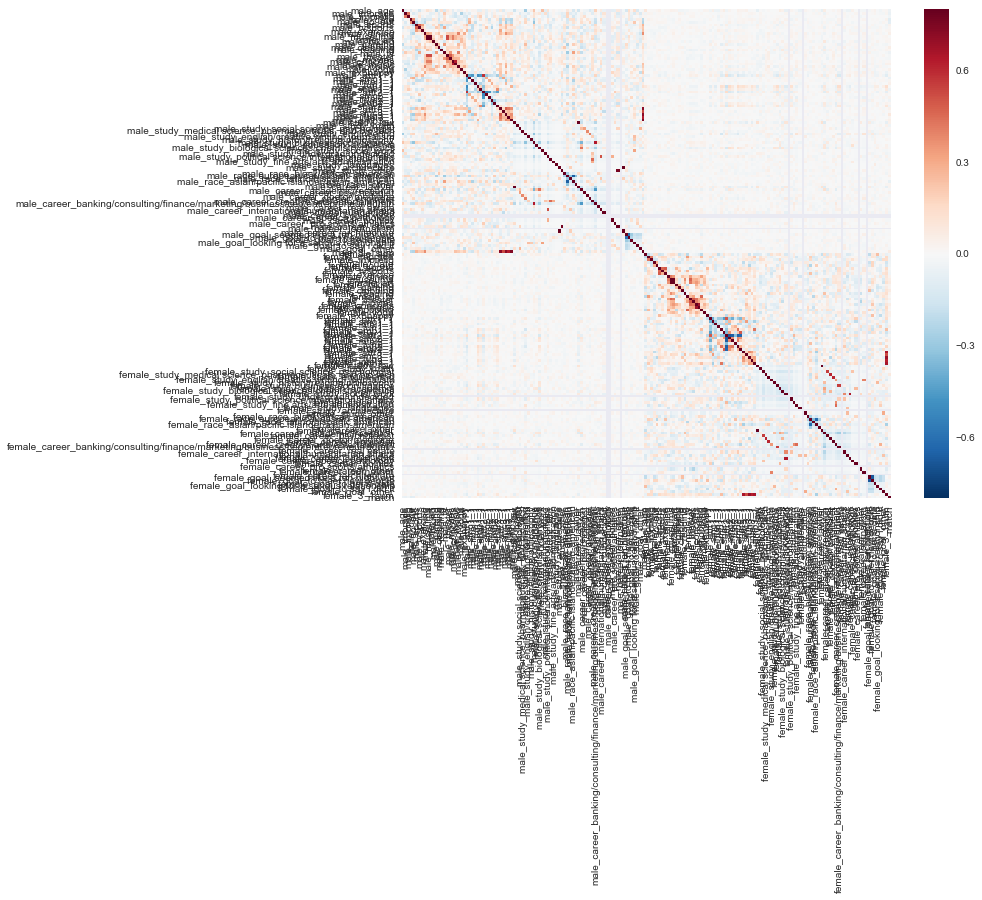
\includegraphics[width=15cm]{img/full_colormap.png}
    \caption{全ての項目間でのヒートマップ}
  \end{center}
\end{figure}
このヒートマップでは項目が多すぎてどの項目がmatchと相関関係にあるのか目視では確認できないが、変数間にも正もしくは負の相関関係があるもの
(正の相関関係は赤で、負の相関関係は青で表現される)と全く相関のないもの(灰色で表現される)があり、無駄な入力情報をいくつも保持するより、
ある程度相関のある変数を利用した方がより精度が高くなるのではないかという仮説が立てられる。

match変数と全ての変数で相関係数を求め、相関係数の大きさに基づいてソートすると、以下の図3で表すような変数が相関関係が大きいことがわかる。
\begin{figure}
  \begin{center}
    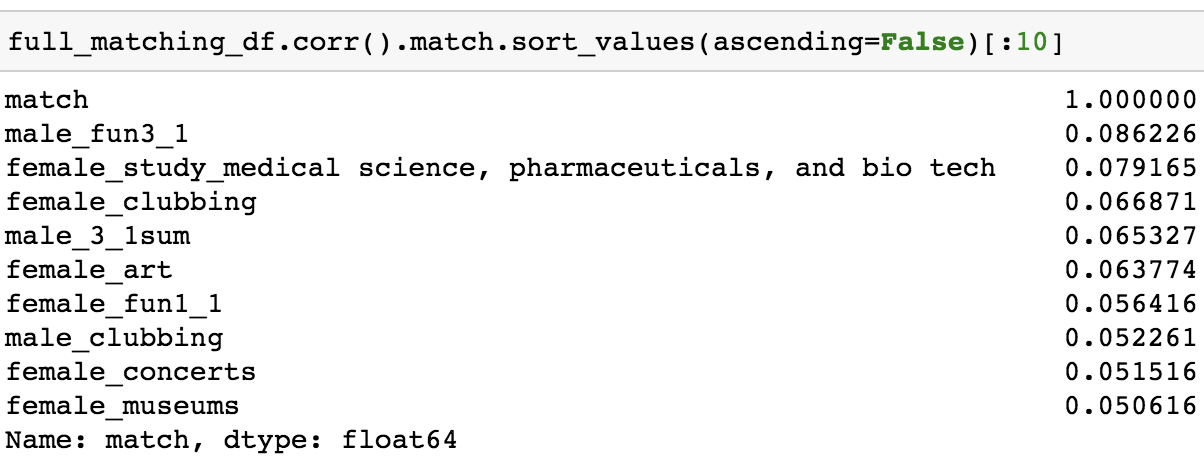
\includegraphics[width=15cm]{img/high_corr.png}
    \caption{match変数と相関の大きい変数の一覧}
  \end{center}
\end{figure}
実際にmatchを除き最も相関が高いとされたmale\_fun3\_1について、マッチングした人を赤、しなかった人を青としてヒストグラムを描画すると、
male\_fun3\_1の値が多いほど、マッチングしたユーザーをマッチングしていないユーザーと比較した時の相対的な割合が大きくなっていることがわかる。
\begin{figure}
  \begin{center}
    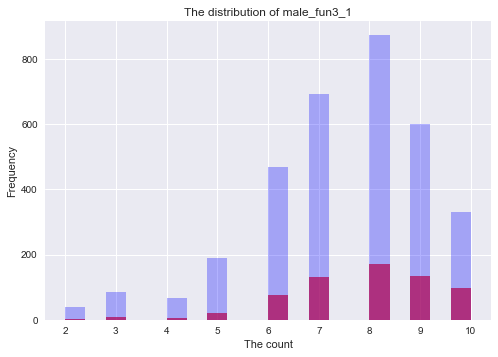
\includegraphics[width=13cm]{img/corr.png}
    \caption{male\_fun3\_1のヒストグラム}
  \end{center}
\end{figure}

以上のような分析の結果、matchとの相関係数の絶対値の大きい18の変数を選択し、
それ以外の変数を入力情報より排除した上でmatchラベルの予測する実験も行なった。

\section{予測結果}
\subsection{学習率、活性化関数を変更し結果を比較する}
まず、二層ニューラルネットワークモデルの学習率、活性化関数を変更し、こういったハイパーパラメータの
変更が結果にどのような影響を与えうるのか観察した。
\begin{description}
  \item[活性化関数の変更]\mbox{}\\
  活性化関数をReLUにした場合及びSigmoidにした場合で、lossの変化の様子、accuracyに変化が現れるか観測した。
  またエポック数は共に10000である。
  \begin{description}
    \item[Sigmoid]\mbox{}\\
    $$h(x) = \frac{1}{1 + \exp{(-x)}}$$
    \item[ReLU]\mbox{}\\
    \[
    h(x) = \begin{cases}
      x & (x > 0) \\
      0 & (x \ leq 0)
    \end{cases}
  \]
  \end{description}
  結果は次の通りになる。
  \begin{table}[htb]
    \centering
    \caption{活性化関数ごとのaccuracy及びlossの比較}
    \begin{tabular}{|c||c|c|c|} \hline
      活性化関数 & training accuracy &  test accuracy & loss \\ \hline \hline
      Sigmoid & 0.841 & 0.826 & 0.604 \\ \hline
      ReLU & 0.835 & 0.842 & 0.424 \\ \hline
    \end{tabular}
  \end{table}
  表1より、ReLUの方がテストデータに対するaccuracyが高く、またlossについても10000エポック終了時
  により小さくなっていることが確認できる。また次の二つの図はSigmoid及びReLUでのlossの推移を観測したものであり、
  Sigmoidについてはエポックが進んでもlossが上昇するなど、値がうまく収束いていないことがわかる。
  \begin{figure}[htbp]
  \begin{minipage}{0.5\hsize}
   \begin{center}
    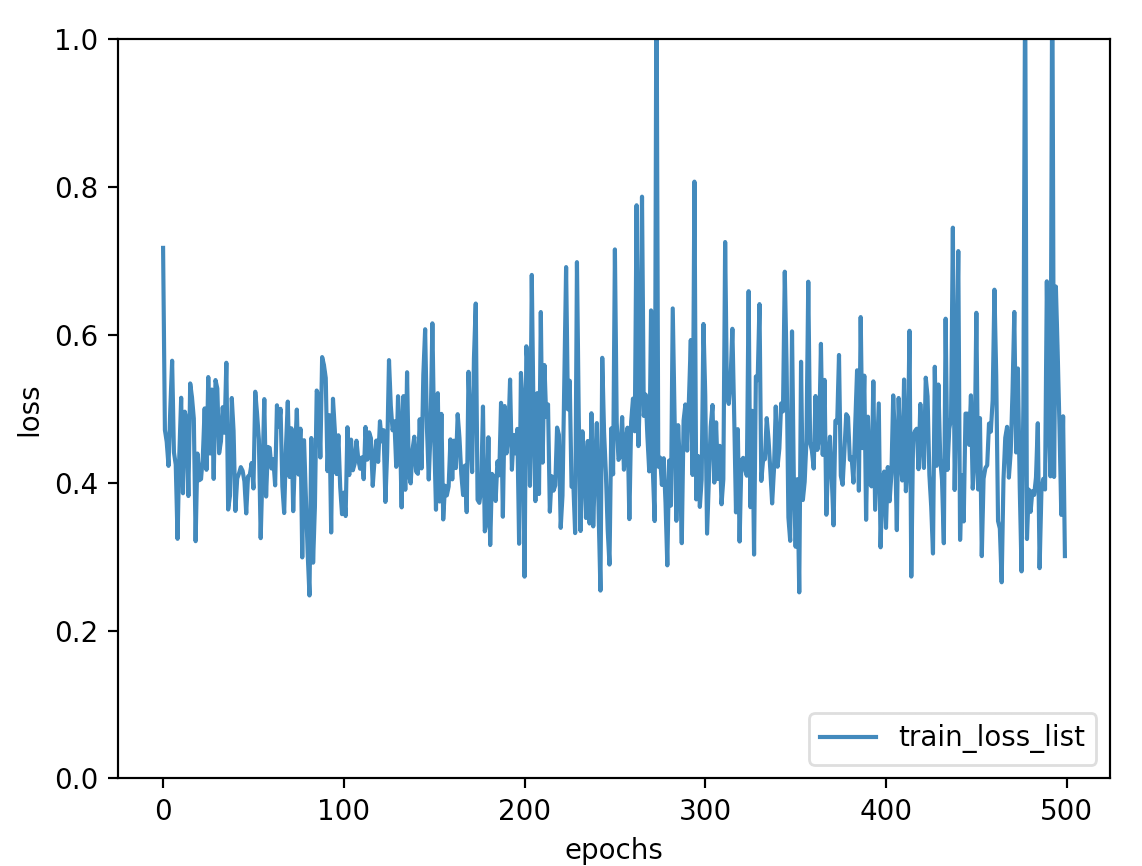
\includegraphics[width=80mm]{img/sigmoid.png}
   \end{center}
   \caption{Sigmoidを活性化関数に用いた時のlossの推移}
   \label{fig:one}
  \end{minipage}
  \begin{minipage}{0.5\hsize}
   \begin{center}
    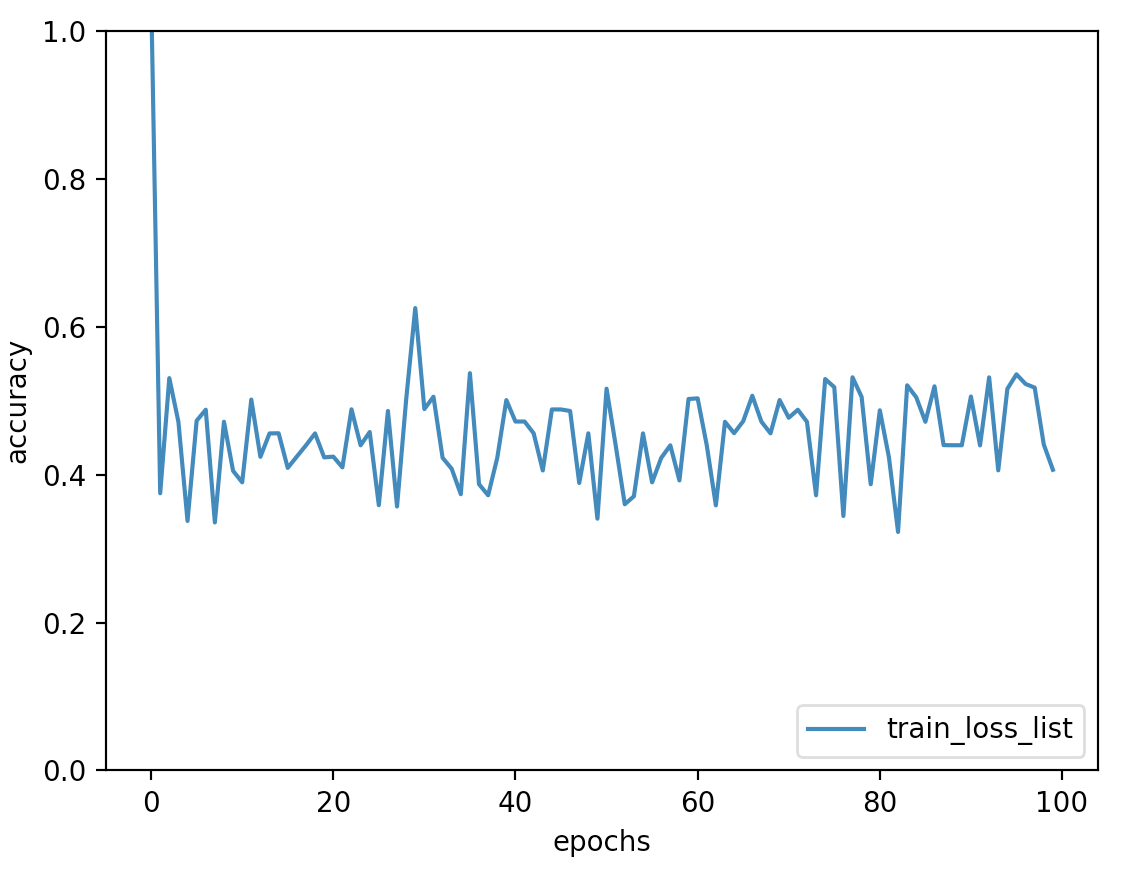
\includegraphics[width=80mm]{img/feature_selection.png}
   \end{center}
   \caption{ReLUを活性化関数に用いた時のlossの推移}
   \label{fig:two}
  \end{minipage}
  \end{figure}


  \item[学習率の変更]\mbox{}\\
  学習率を0.1, 0.5, 1.0と変化した時の最終エポック時のaccuracy及びlossの値は次のようになった。
  \begin{table}[htb]
    \centering
    \caption{学習率を変化させた時のaccuracy及びlossの比較}
    \begin{tabular}{|c||c|c|c|} \hline
      学習率 & training accuracy &  test accuracy & loss \\ \hline \hline
      0.1 & 0.838 & 0.833 & 0.439 \\ \hline
      0.5 & 0.834 & 0.842 & 0.460 \\ \hline
      1.0 & 0.834 & 0.843 & 0.387 \\ \hline
    \end{tabular}
  \end{table}
\end{description}
表2の結果を見ると、学習率については少なくとも今回のタスクにおいてはあまり大きく結果に影響を与えているわけではないように見受けられる。

\subsection{特徴選択の有無}
特徴選択を有りにした(すなわち入力変数の数を20以下に制限した)時と全ての特徴を入力変数として用いた時の
パフォーマンス及び計算時間の比較を行なった。
\begin{table}[htb]
  \centering
  \caption{学習率を変化させた時のaccuracy及びlossの比較}
  \begin{tabular}{|c||c|c|c|c|} \hline
    特徴選択 & training accuracy &  test accuracy & loss & 計算時間[sec]\\ \hline \hline
    有り & 0.831 & 0.851 & 0.487 & 19.76 \\ \hline
    無し & 0.834 & 0.843 & 0.460 & 44.51 \\ \hline
  \end{tabular}
\end{table}
% \end{description}
表3のように、特徴選択は精度の向上にある程度貢献しているように思われる。また特筆すべきは計算時間で有り、
特徴選択を行なった場合、50000エポックにかかる時間が特徴選択を行わない場合と比較し半分以下となっている。
精度の面でも上回るもしくは差異がない程度であれば、ある程度使用する特徴を絞ってしまった方が
特に計算時間になんらかの制約条件がある場合は良いのではないかと感じた。

% \begin{thebibliography}{9}
%   \bibitem{evans} Andreas Holzinger, David Blanchard, Vasile Palade, Raul Rabadan.
%     "Darwin, Lamarck, or Baldwin: Applying Evolutionary Algorithms to Machine Learning Techniques",  IEEE/WIC/ACM International Joint Conferences on Web Intelligence (WI) and Intelligent Agent Technologies (IAT), 2014.
% \end{thebibliography}


\end{document}
